\documentclass[12pt, a4paper]{article}
\usepackage{import}
\usepackage{preamble}

\title{Regression and Curve Fitting}
\date{6\(^\text{{th}}\) October 2022}
\author{Lee Farrugia}

\begin{document}
    
\maketitle
\thispagestyle{titlepagestyle}
\pagestyle{mystyle}

\section*{Task 1 - Simple Linear Regression}
\subsection*{Abstract}
insert very important stuff here

\subsection*{Introduction and Theoretical Background}
cause why the fuck not

\subsection*{Materials and Methods}

\subsubsection*{Languages and Packages}
Python 3.10.8, Pandas, Numpy, Matplolib.pyplot.

\subsubsection*{Methodology}
\begin{enumerate}
    \item The dataset provided was imported into the program, each variable defined according to its respective column of data, and each variable was converted into an array with the use of numpy.
    \item A function was constructed to calculate the \(\alpha\) and \(\beta\) that correspond to the \(\alpha\) and \(\beta\) of the equation:
    \begin{equation}
        Y_e = \alpha + \beta X .
    \end{equation}
    \(\alpha\) and \(\beta\) were further defined as the following:
    \begin{align}
        \beta &= \frac{\sum_{i=1}^{n}(X_i - \bar{X})(Y_i - \bar{Y})}{\sum_{i=1}^{n}(X_i - \bar{X})^2} ,\\
        \alpha &= \bar{Y} - \beta \bar{X} .
    \end{align}
    \item This function was further expanded to include the calculation of the uncertainties of \(\alpha\) and \(\beta\), and the correlation coefficient and coefficient of determination.
    \item Using this function the experimental values for \(E\) and \(T_0\) and their respective uncertainties were calculated. Using these values a trendline was generated, with the residuals being plotted directly underneath it. 
\end{enumerate}

\subsection*{Results}

\subsection*{Discussion}

\subsection*{Figures and Graphs}
\begin{figure}[H]
    \centering
    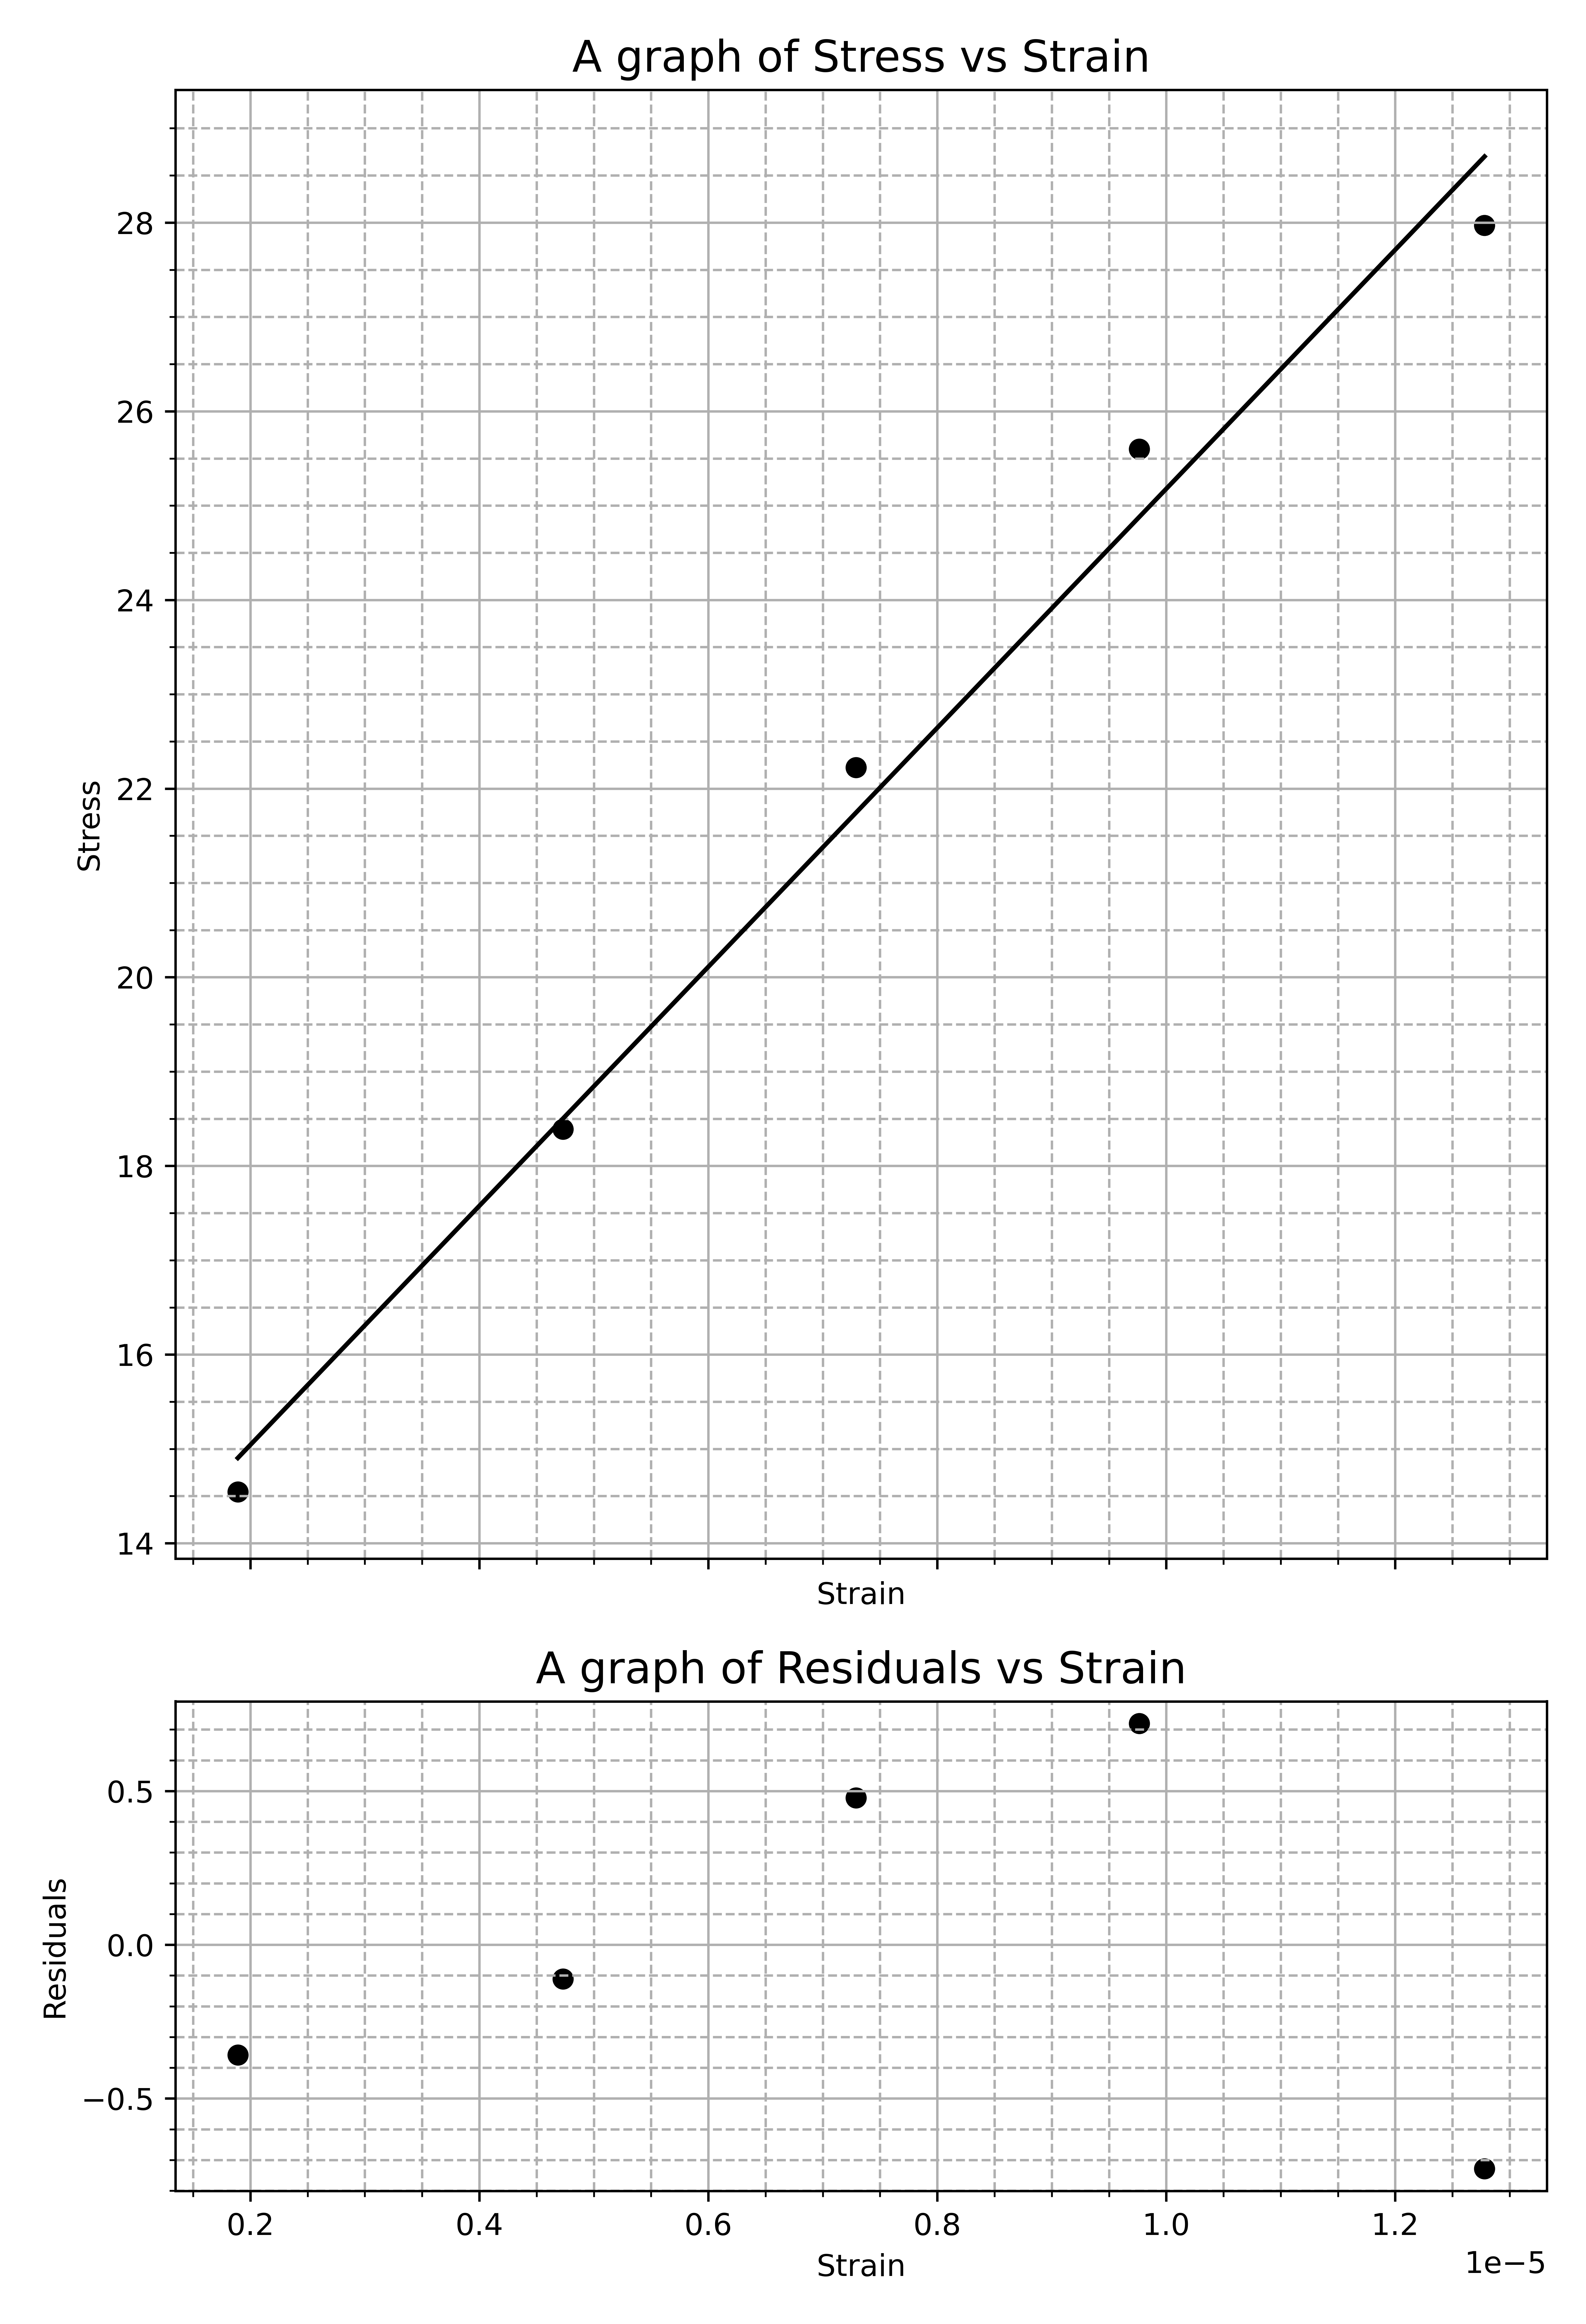
\includegraphics[width = \textwidth]{1Plot1.png}
    \caption{A graph of stress vs strain and their respective residuals}
\end{figure}

\begin{figure}[H]
    \centering
    \includegraphics[width = \textwidth]{2Plot1.png}
    \caption{A graph of Luminosity vs Temperature}
\end{figure}

\begin{figure}[H]
    \centering
    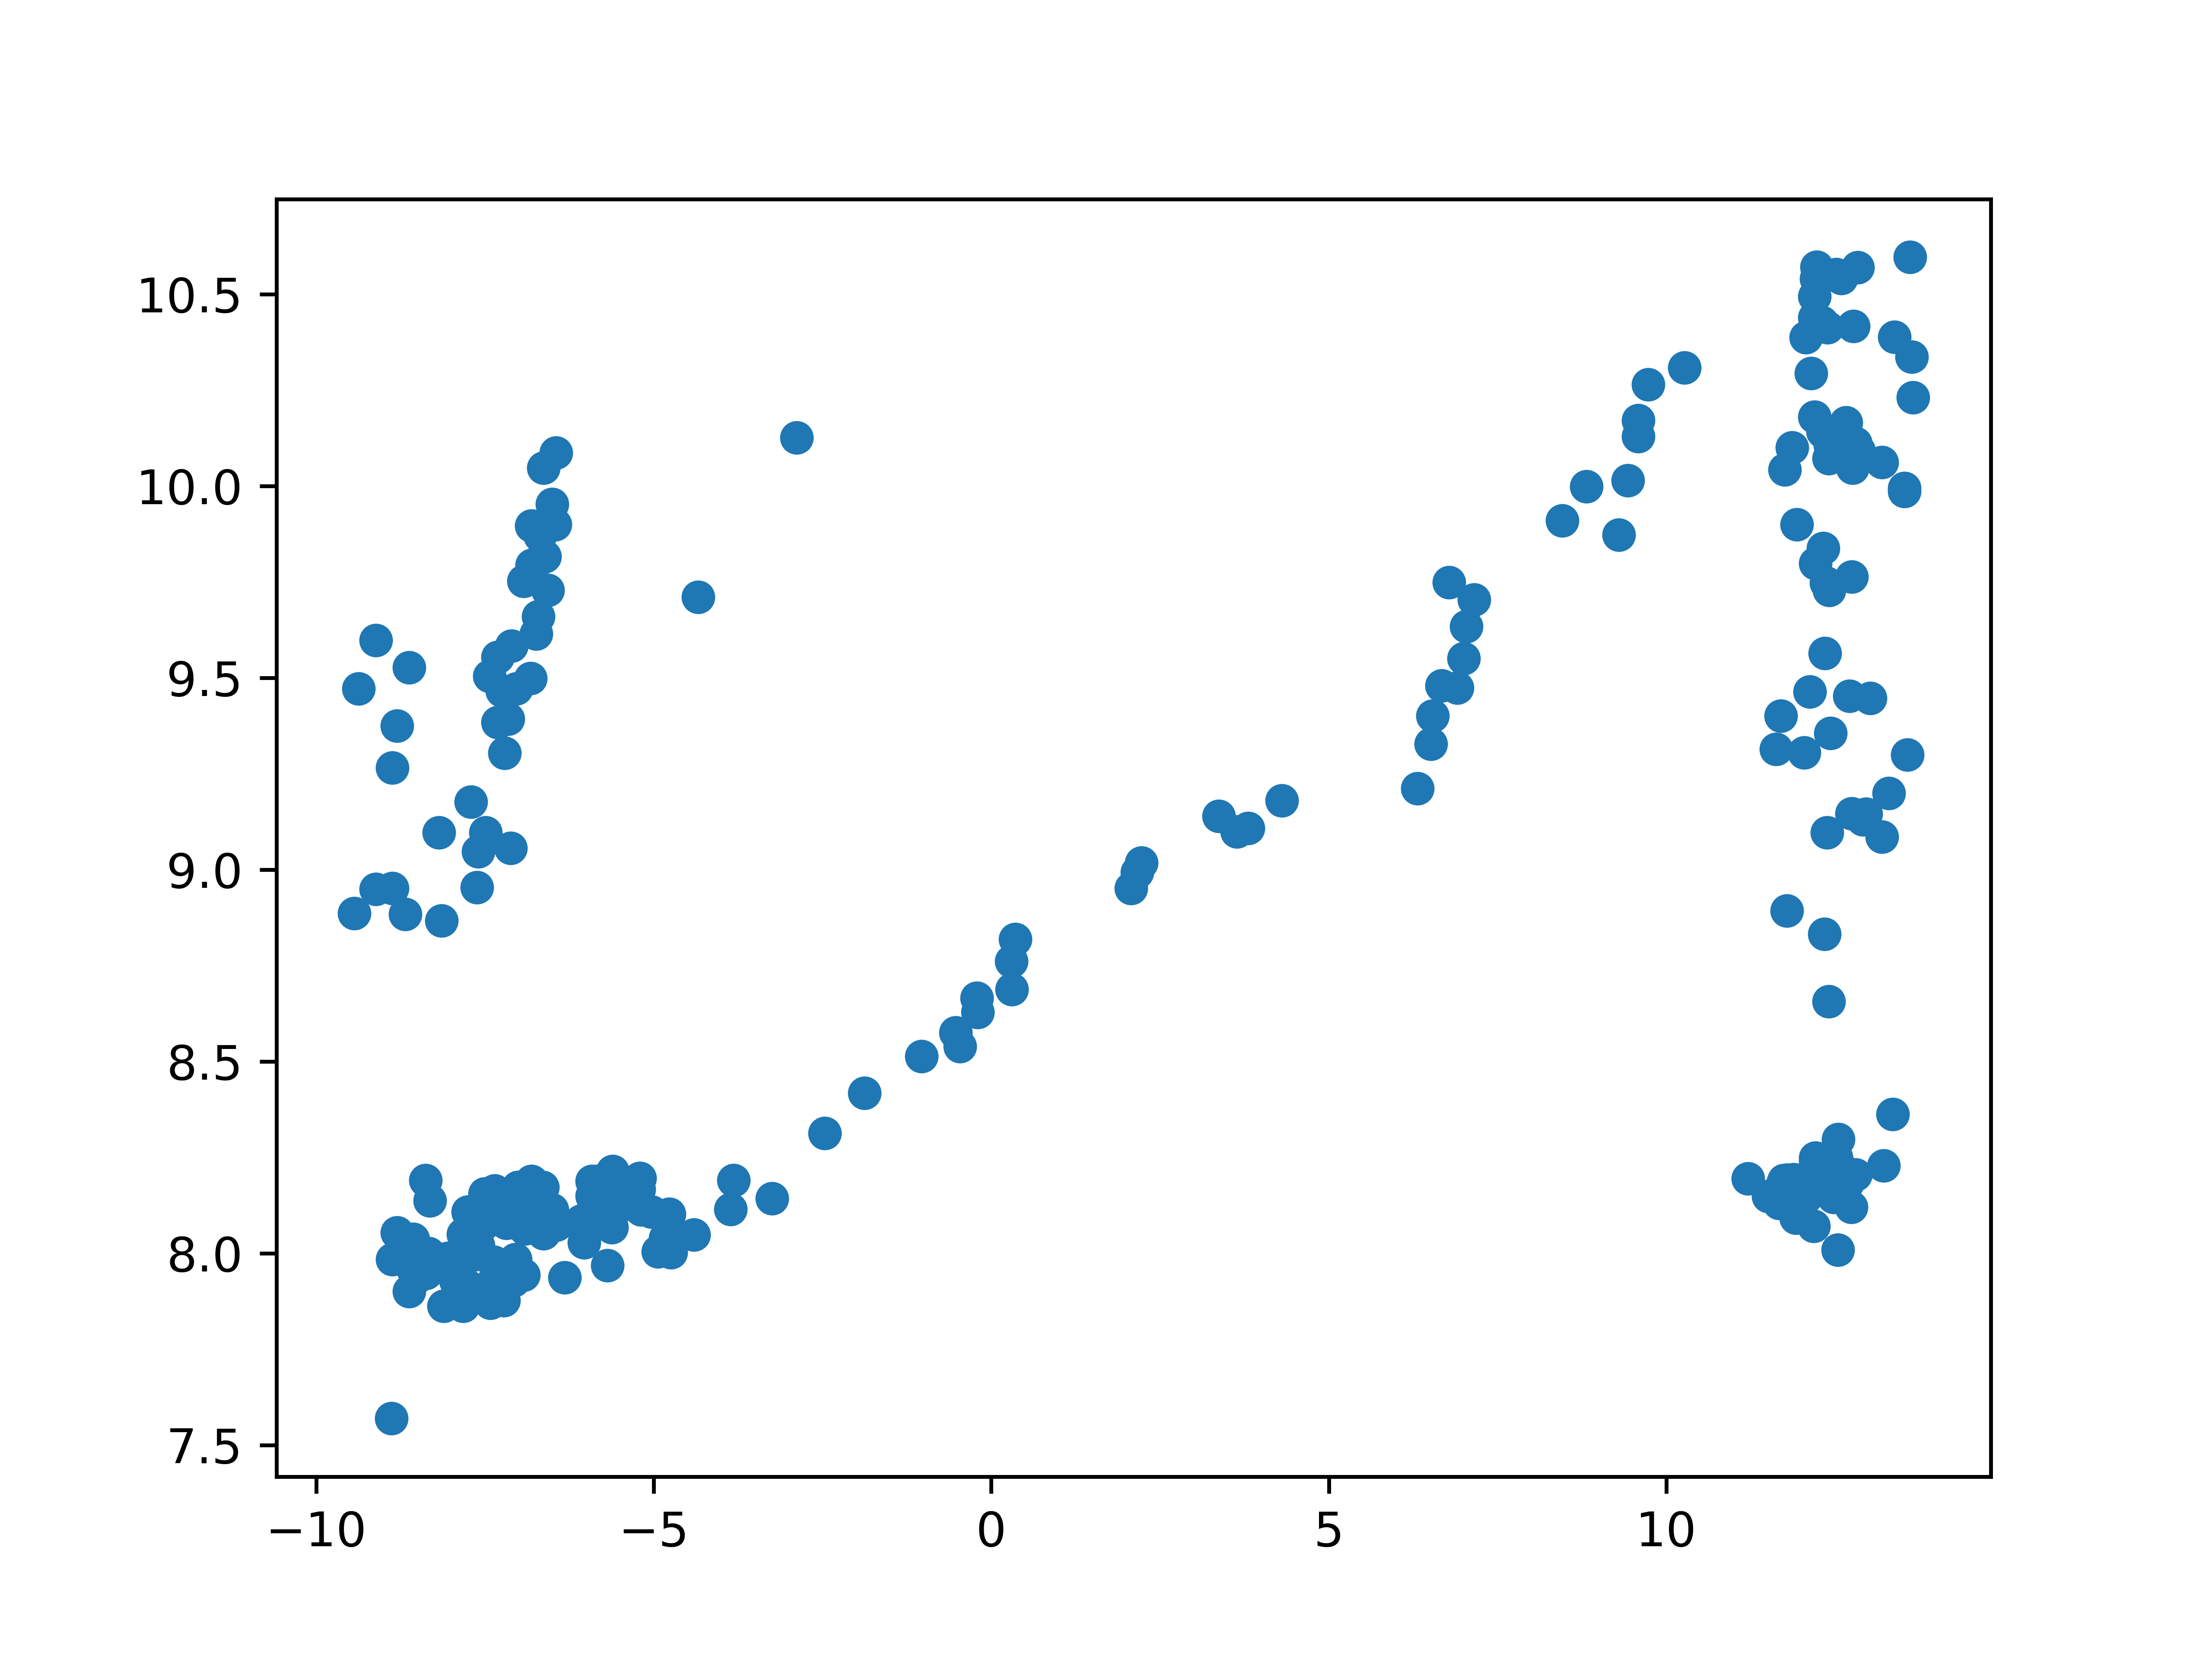
\includegraphics[width = \textwidth]{2Plot2.png}
    \caption{A graph of \(\log{Luminosity}\) vs \(\log{Temperature}\)}
\end{figure}

\begin{figure}[H]
    \centering
    \includegraphics[width = \textwidth]{2Plot3.png}
    \caption{A graph of \(\log{Luminosity}\) vs \(\log{Temperature}\) for star type 3}
\end{figure}

\begin{figure}[H]
    \centering
    \includegraphics[width = \textwidth]{2Plot4_2.png}
    \caption{A graph of \(\log{Luminosity}\) vs \(\log{Temperature}\) for star type 3, with degree 2}
\end{figure}

\begin{figure}[H]
    \centering
    \includegraphics[width = \textwidth]{2Plot4_10.png}
    \caption{A graph of \(\log{Luminosity}\) vs \(\log{Temperature}\) for star type 3, with degree 10}
\end{figure}

\begin{figure}[H]
    \centering
    \includegraphics[width = \textwidth]{2Plot4_15.png}
    \caption{A graph of \(\log{Luminosity}\) vs \(\log{Temperature}\) for star type 3, with degree 15}
\end{figure}

\begin{figure}[H]
    \centering
    \includegraphics[width = \textwidth]{2Plot4_16.png}
    \caption{A graph of \(\log{Luminosity}\) vs \(\log{Temperature}\) for star type 3, with degree 16}
\end{figure}

\begin{figure}[H]
    \centering
    \includegraphics[width = \textwidth]{2Plot4_17.png}
    \caption{A graph of \(\log{Luminosity}\) vs \(\log{Temperature}\) for star type 3, with degree 17}
\end{figure}

\begin{figure}[H]
    \centering
    \includegraphics[width = \textwidth]{2Plot4_20.png}
    \caption{A graph of \(\log{Luminosity}\) vs \(\log{Temperature}\) for star type 3, with degree 20}
\end{figure}

\begin{figure}[H]
    \centering
    \includegraphics[width = \textwidth]{2Plot4_25.png}
    \caption{A graph of \(\log{Luminosity}\) vs \(\log{Temperature}\) for star type 3, with degree 25}
\end{figure}

\begin{figure}[H]
    \centering
    \includegraphics[width = \textwidth]{2Plot4_30.png}
    \caption{A graph of \(\log{Luminosity}\) vs \(\log{Temperature}\) for star type 3, with degree 30}
\end{figure}

\begin{figure}[H]
    \centering
    \includegraphics[width = \textwidth]{2Plot5.png}
    \caption{A graph of \(\frac{L}{a}\) vs T}
\end{figure}

\begin{figure}[H]
    \centering
    \includegraphics[width = \textwidth]{3Plot1.png}
    \caption{A graph of \(\log{A}\) vs \(\log{T}\)}
\end{figure}

\begin{figure}[H]
    \centering
    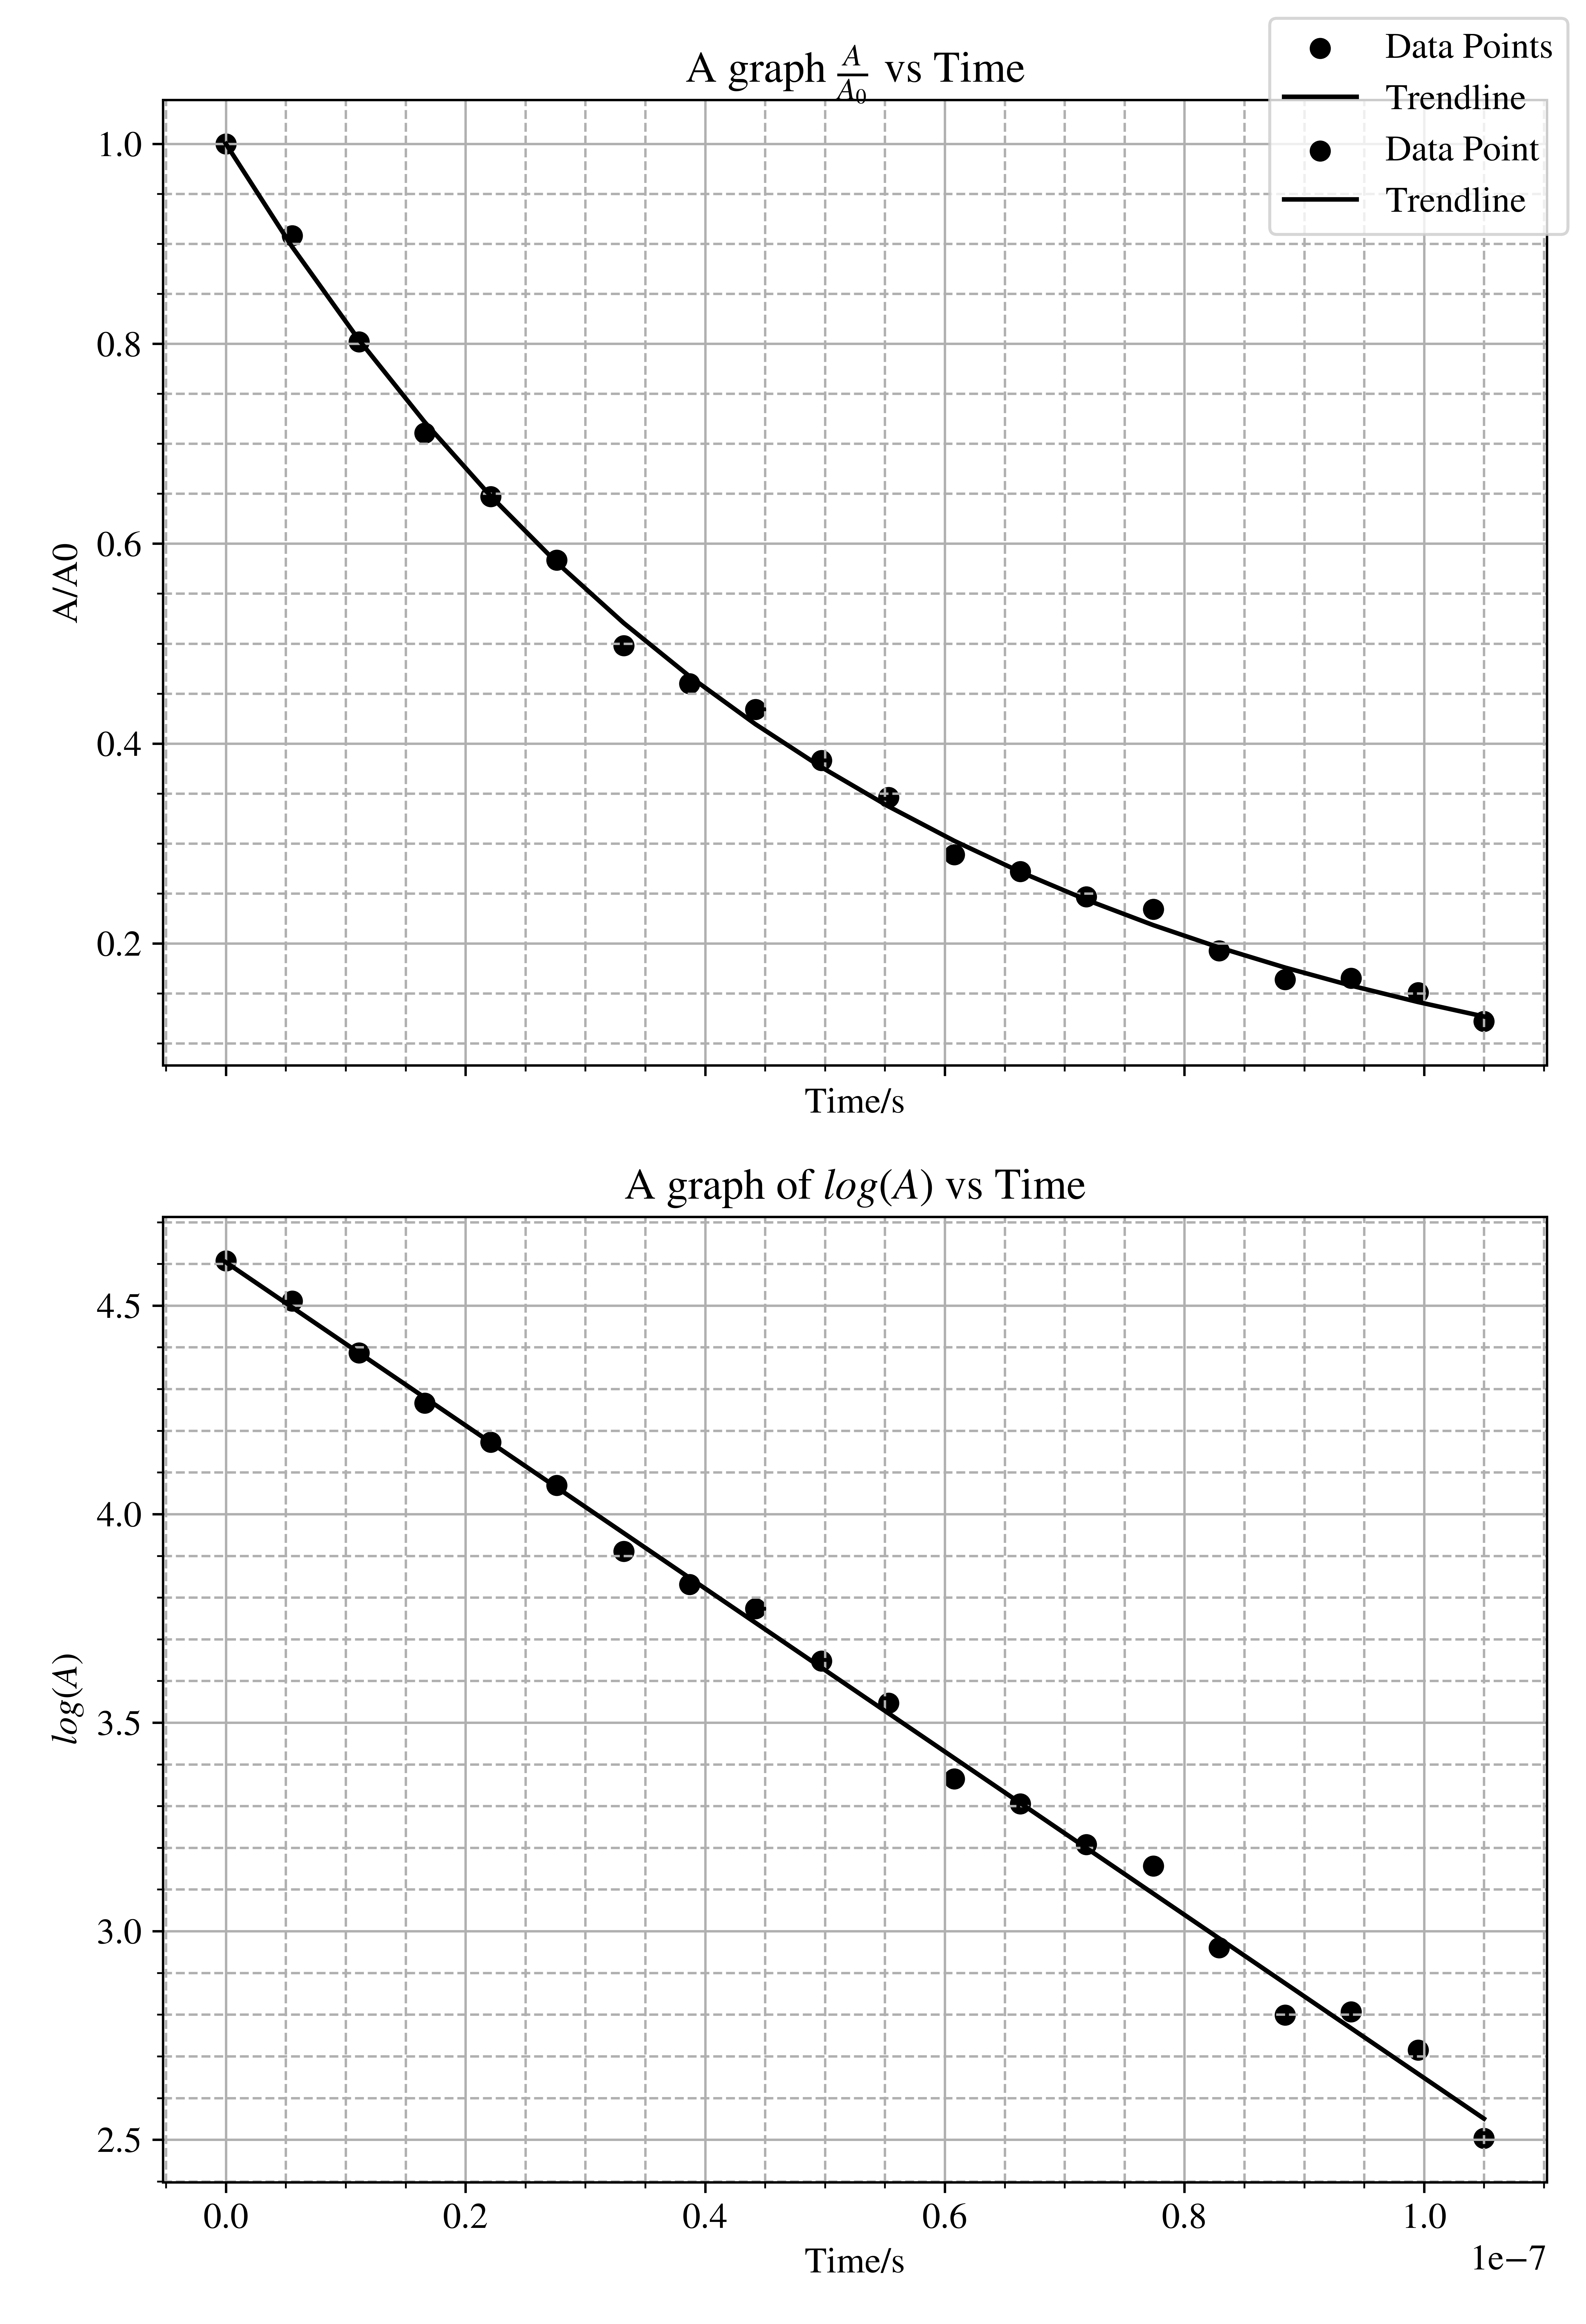
\includegraphics[width = \textwidth]{3Plot2.png}
    \caption{A graph of \(\frac{A}{A_0}\) vs T and subplot of \(\log{A}\) vs \(\log{T}\)}
\end{figure}

\begin{figure}[H]
    \centering
    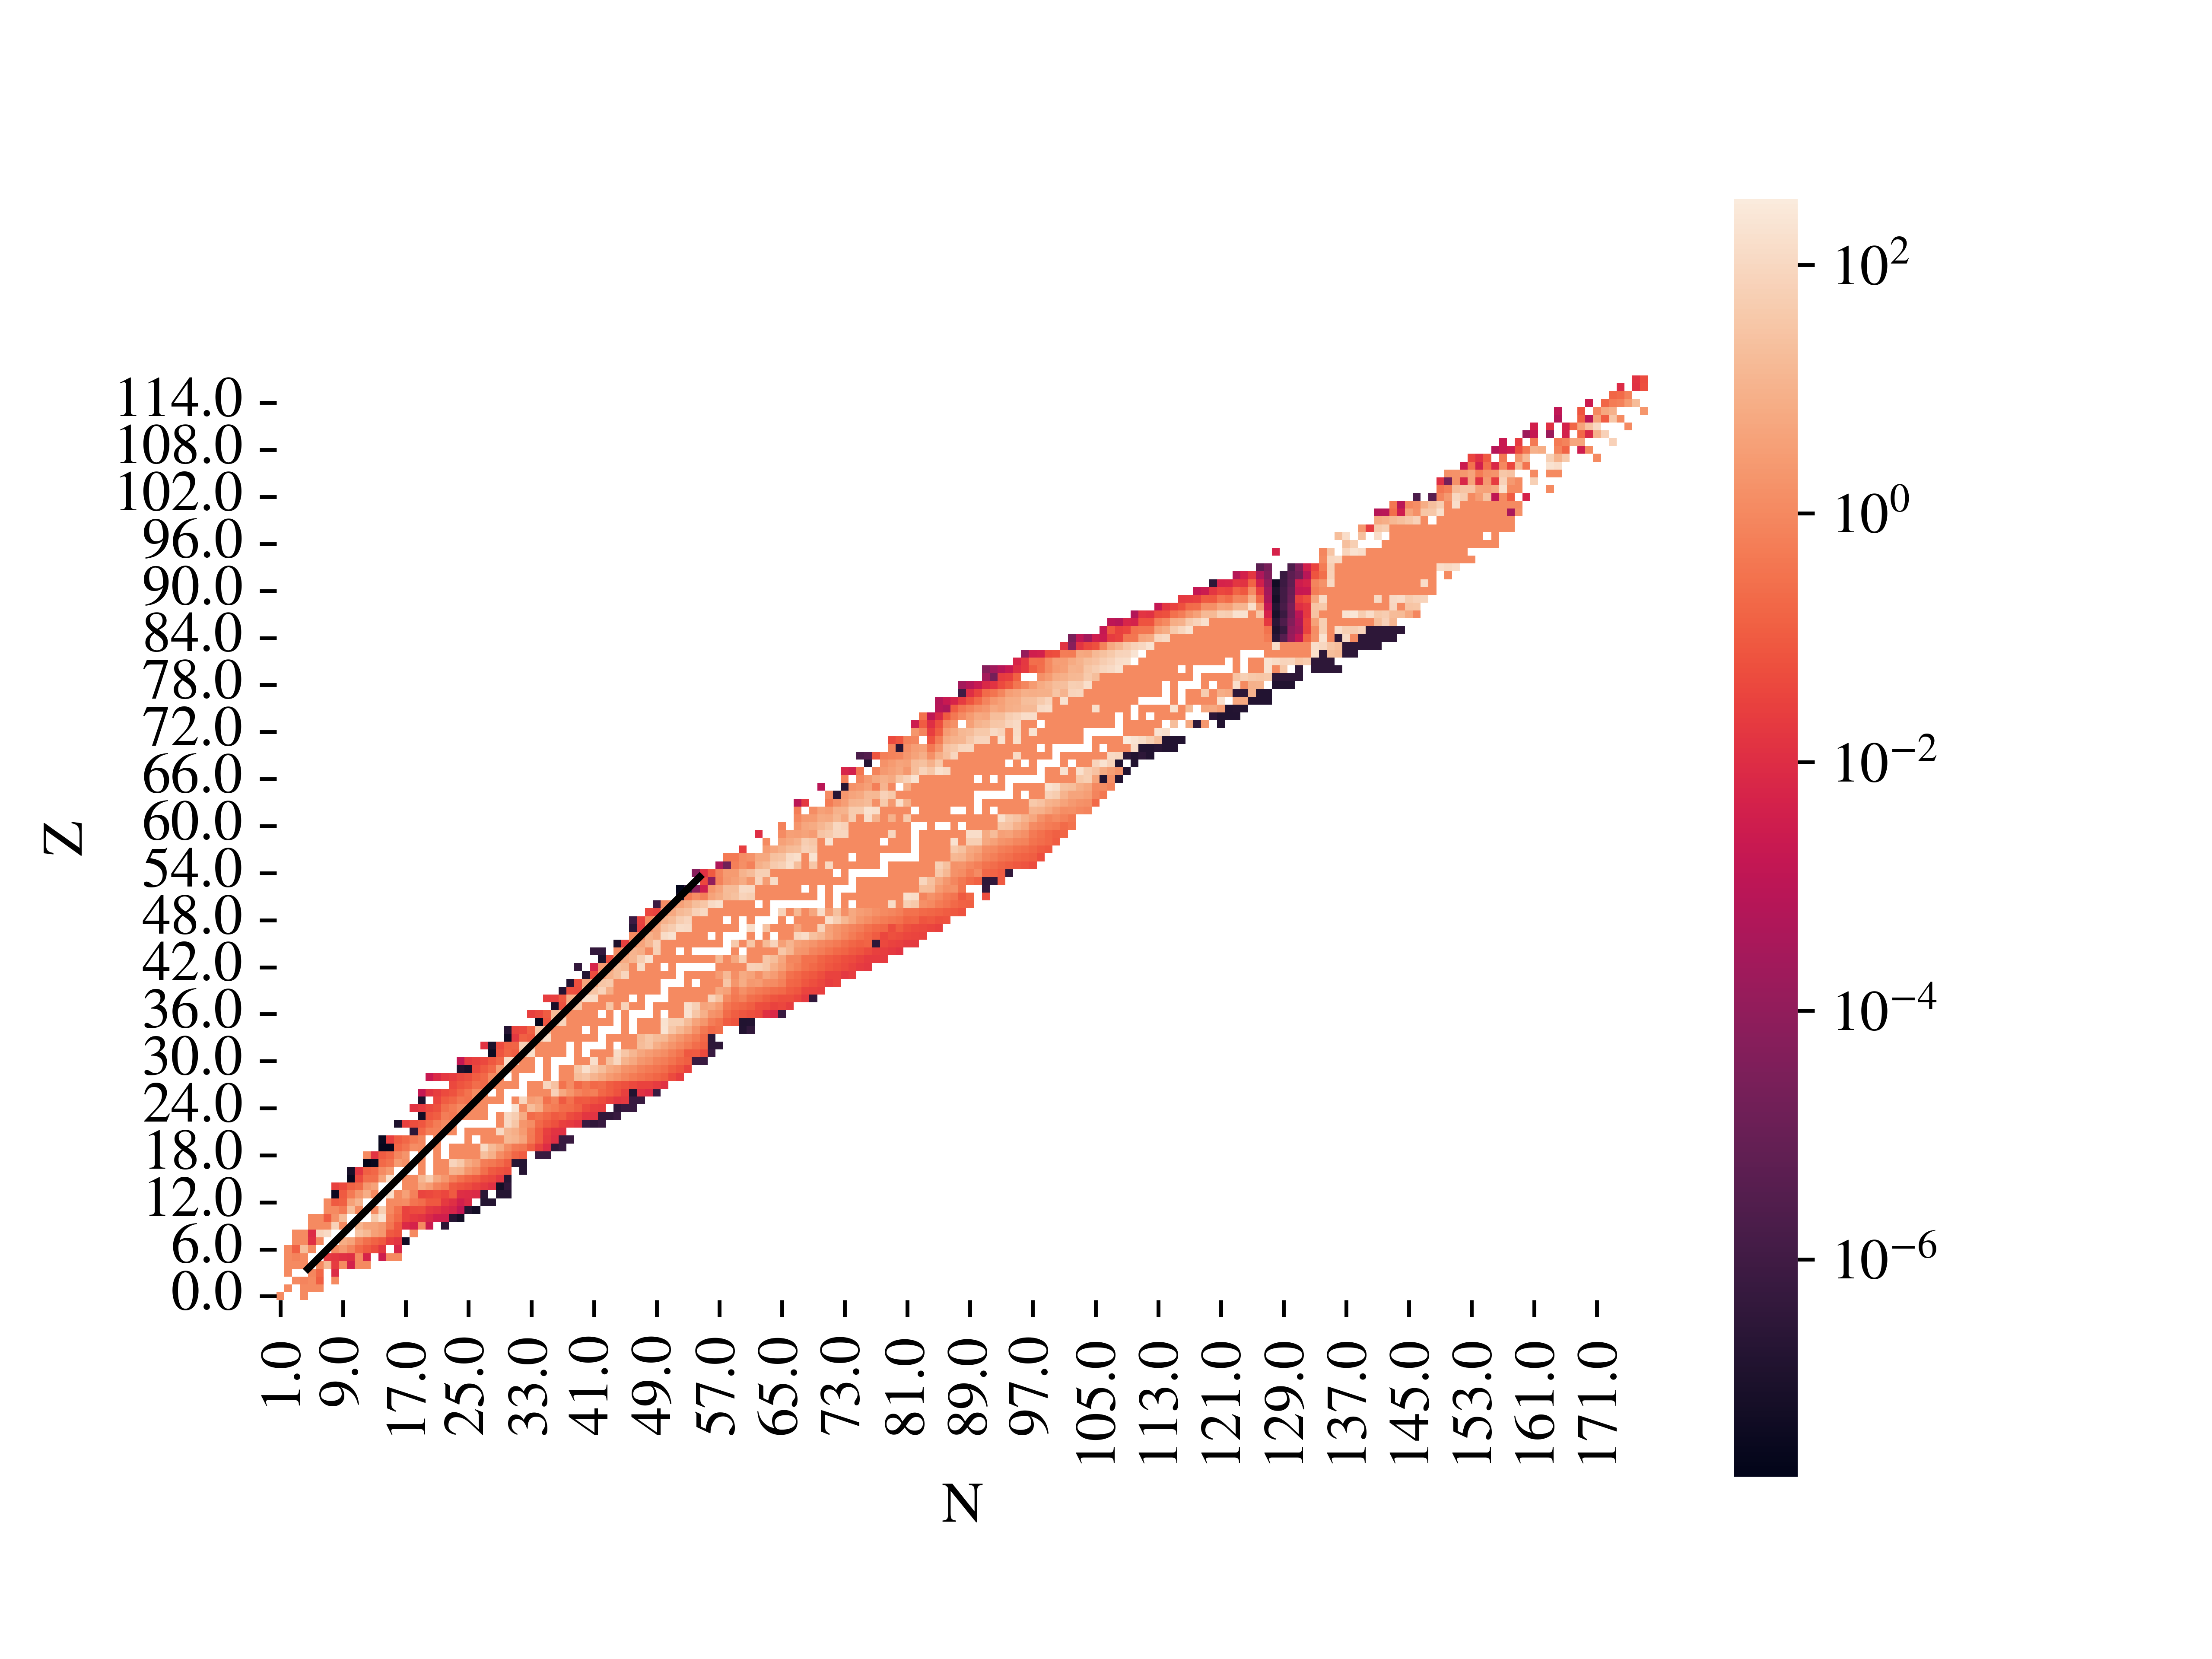
\includegraphics[width = \textwidth]{3Plot3.png}
    \caption{A heat map of the Z vs N with the stability line}
\end{figure}

\begin{figure}[H]
    \centering
    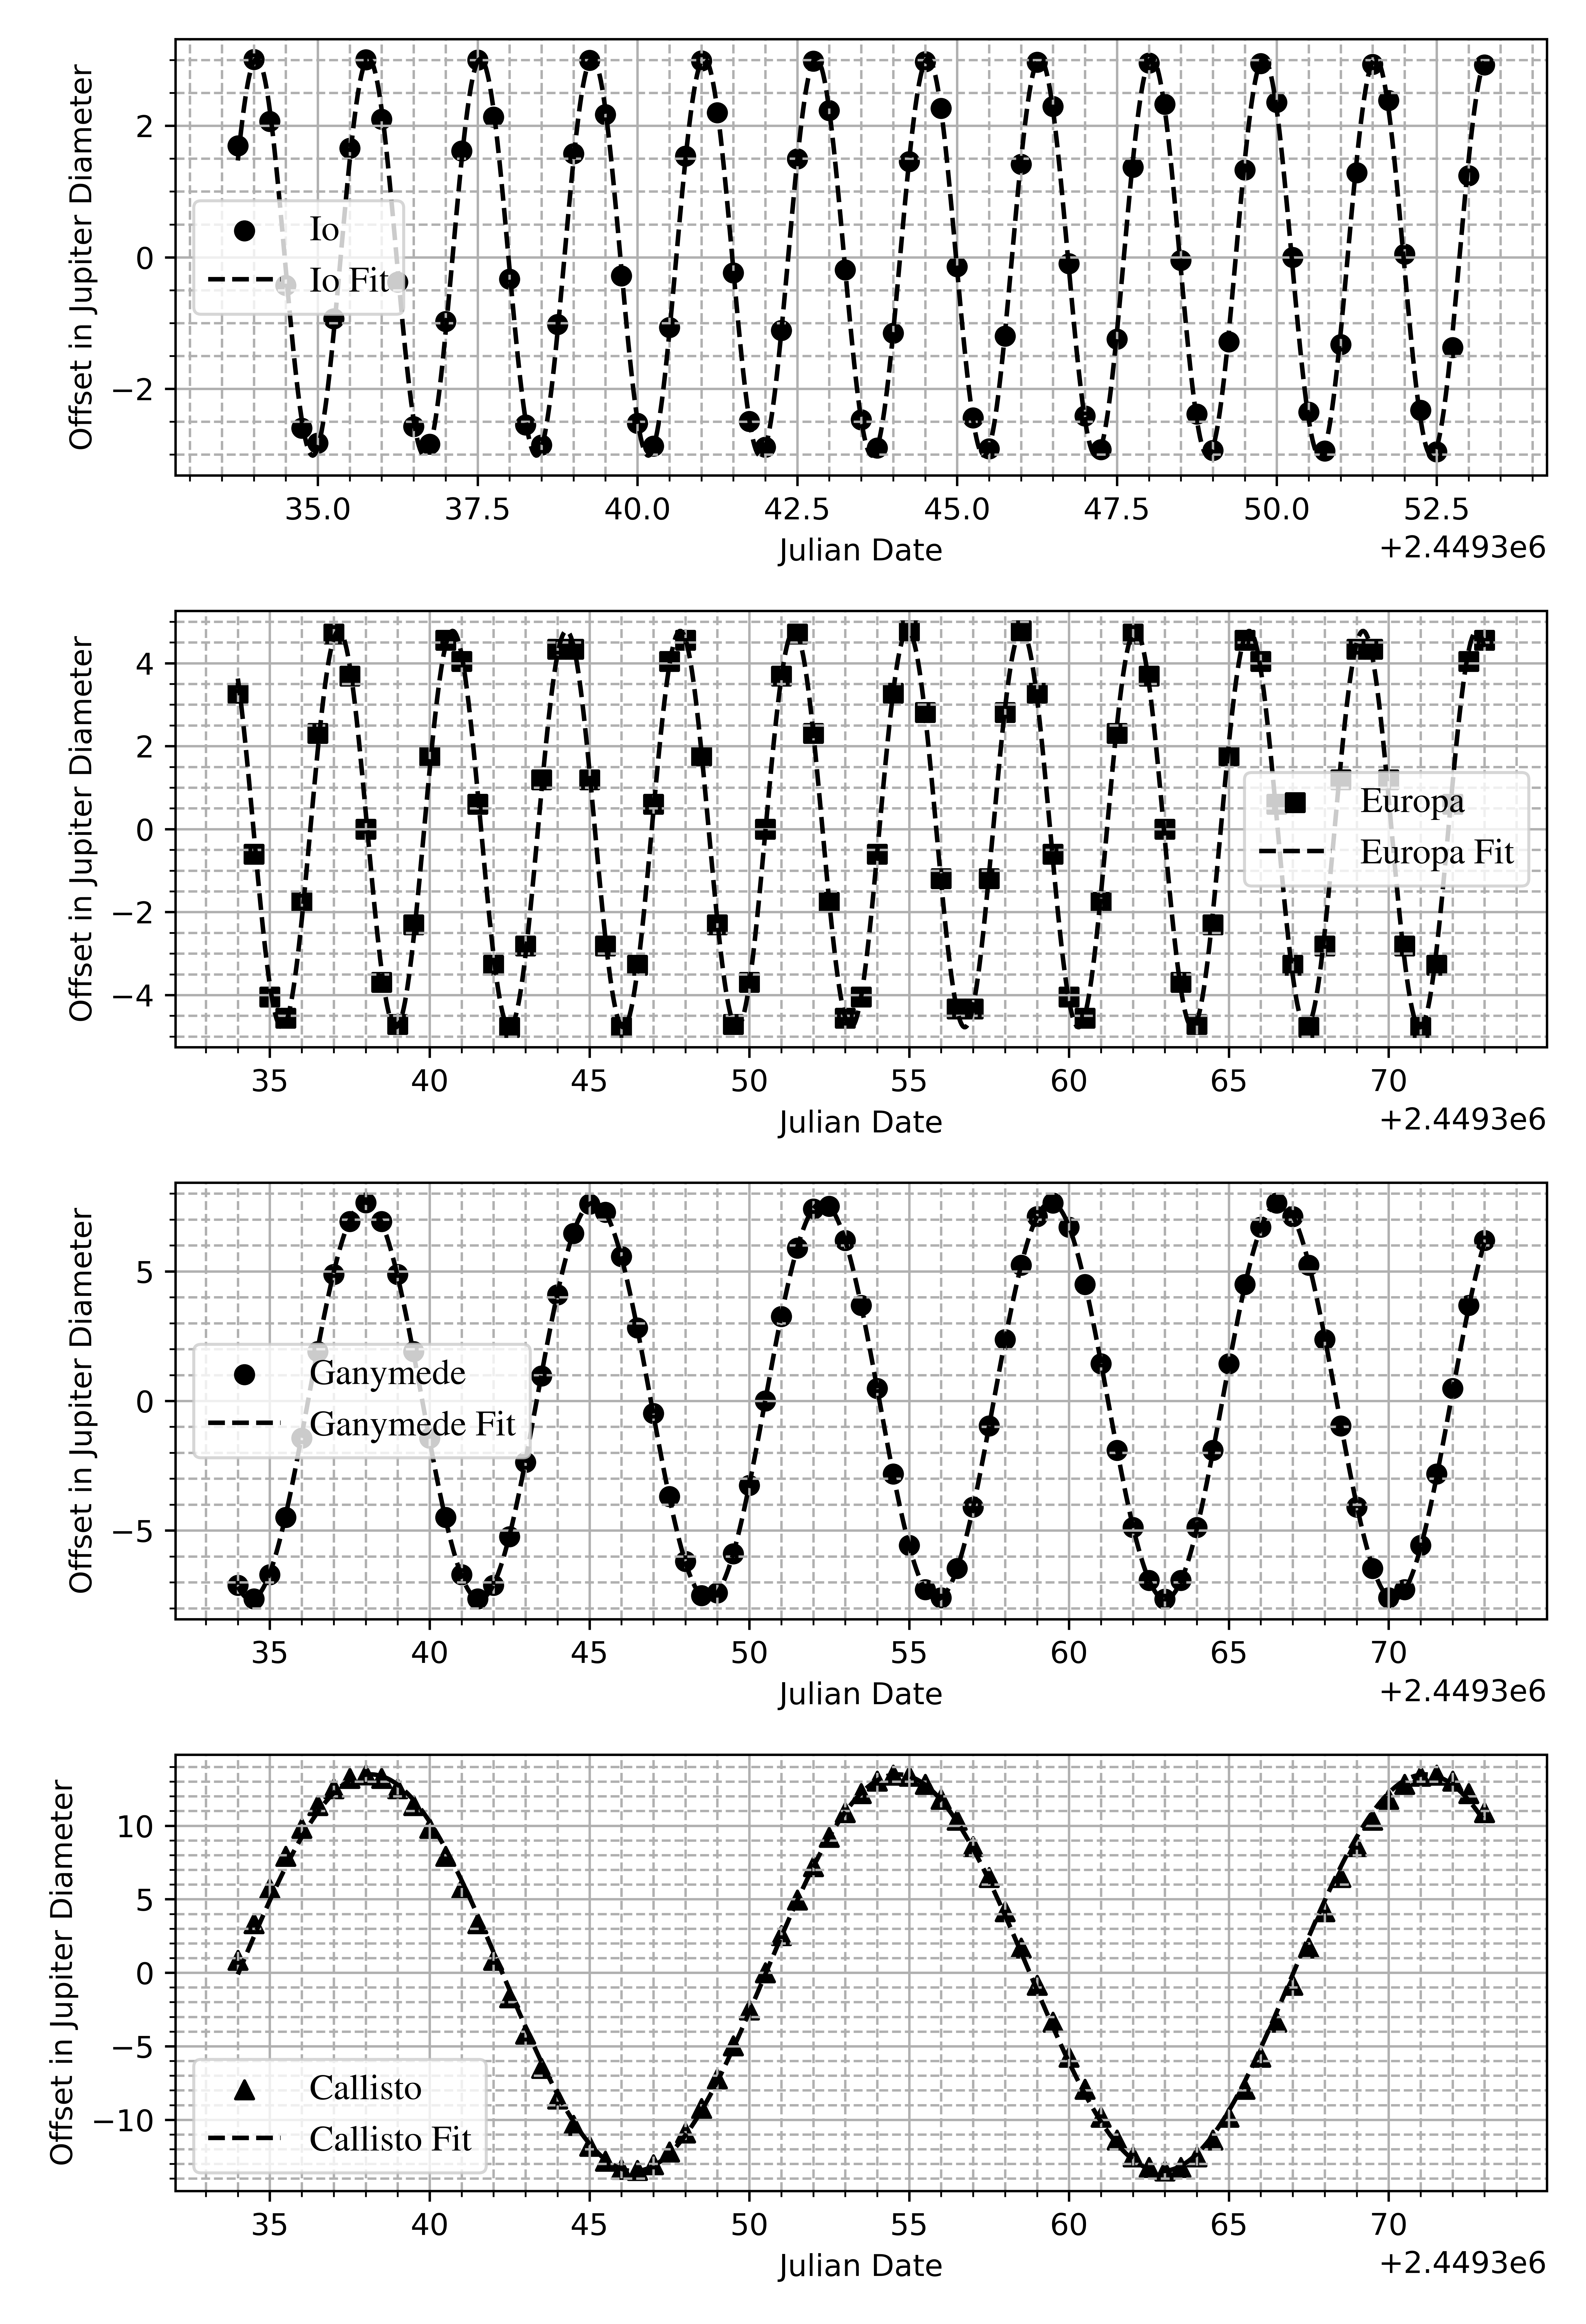
\includegraphics[width = \textwidth]{4Plot1.png}
    \caption{A graph of all moon offset vs julian date waves}
\end{figure}

\begin{figure}[H]
    \centering
    \includegraphics[width = \textwidth]{4Plot2.png}
    \caption{A graph of \(r^3\) vs \(T^2\)}
\end{figure}

\section*{Appendix}
\begin{minted}{py}
# Task 1

import numpy as np
import pandas as pd
import matplotlib.pyplot as plt

# creating the empty lists to be used
xlist = []
ylist = []
prodlist = []
denomlist = []
ydenomlist = []
yelist = []

# reading the data
data = pd.read_csv('Q1__Youngs_Modulus_of_a_Wire.csv')
# changing the individual columns into arrays
diameter_array = (data['Diameter/m']).to_numpy()
mass_array = data['m/kg'].to_numpy()
x1_array = data['x_1/m'].to_numpy()
x2_array = data['x_2/m'].to_numpy()
x3_array = data['x_3/m'].to_numpy()
x4_array = data['x_4/m'].to_numpy()
L_array = data['L/m'].to_numpy()
x0_array = data['x_0/m'].to_numpy()

# finding the x-x0 part of the equation
for i in range(len(x1_array)-1):
    x = sum([x1_array[i], x2_array[i], x3_array[i], x4_array[i]])
    X = (x/4)-x0_array[0]
    xlist.append(abs(X))

# calculating xi and xbar
xi = np.array(xlist)**2
xbar = np.mean(xi)

# calculating yi and y bar
for i in range(len(mass_array)-1):
    yi = mass_array[i]/xlist[i]
    ylist.append(yi)

yi = np.array(ylist)
ybar = np.mean(yi)

# defining the function to calculate alpha, beta, coefficient of correlation and determination
def beta_alpha_function(xi, xbar, yi, ybar):
    for i in range(len(xi)):
        prod = (xi[i]-xbar)*(yi[i]-ybar)
        prodlist.append(prod)
        xdenom = (xi[i]-xbar)**2
        denomlist.append(xdenom)
        ydenom = (yi[i]-ybar)**2
        ydenomlist.append(ydenom)
    prod_array = np.array(prodlist)
    denom_array = np.array(denomlist)
    ydenom_array = np.array(ydenomlist)
    numerator = sum(prod_array)
    denominator = sum(denom_array)
    ydenominator = sum(ydenom_array)
    beta = numerator/denominator
    alpha = ybar - (beta*xbar)
    r = numerator/(np.sqrt(denominator*ydenominator))
    delta_beta = (beta/(np.sqrt(len(xi)-2)))*(np.sqrt((1/r**2)-1))
    delta_alpha = delta_beta*np.sqrt(((1/len(xi))*(sum(xi**2))))
    R = r**2
    return beta, alpha, delta_beta, delta_alpha, r, R

# calling previous function to get the actual values
beta, alpha, delta_beta, delta_alpha, r, R = beta_alpha_function(xi, xbar, yi, ybar)

# calculating the experimental values 
for i in range(len(xi)):
    ye = alpha + (beta*xi[i])
    yelist.append(ye)
ye_array = np.array(yelist)

# calculating the constants for the gradient and intercept
radius = np.average(diameter_array)
m_constant = (8*np.pi*(radius**2))/(9.81*(L_array[0]**3))
c_constant = 4/(L_array[0]*9.81)

# finding the line of best fit to the data
coeffs, cov = np.polyfit(xi, ye_array, 1, cov=True)
polyfunc = np.poly1d(coeffs)
trendline = polyfunc(xi)

# calculating the young's modulus and T0
E = coeffs[0]/m_constant
T0 = coeffs[1]/c_constant
delta_E = np.sqrt(cov[0][0])
delta_T0 = np.sqrt(cov[1][1])
print(f'the value of E is : {E}, with an error of: {delta_E}. The value of T0: {T0}, with and error of {delta_T0}')

# calculating the residuals
residual = np.subtract(yi,trendline)

f, (a0, a1) = plt.subplots(2, 1, sharex=True, sharey=False, gridspec_kw={'height_ratios': [3, 1]}, figsize=(7.3, 10.7))

# defining the font to be used
plt.rcParams['font.family'] = 'STIXGeneral'
plt.rcParams['mathtext.fontset'] = 'stix'
plt.rcParams['font.size'] = 12
plt.rcParams['font.weight'] = 'normal'

# plotting both graph as subplots
a0.scatter(xi, yi, color='k', label='Data Points')
a0.plot(xi, trendline, color='k', label='Trendline')
a0.minorticks_on()
a0.grid(visible=True, which='major', linestyle='-')
a0.grid(visible=True, which='minor', linestyle='--')
a0.set_xlabel('Strain')
a0.set_ylabel('Stress')
a0.set_title('A graph of Stress vs Strain')

a1.scatter(xi, residual, color='k')
a1.minorticks_on()
a1.grid(visible=True, which='major', linestyle='-')
a1.grid(visible=True, which='minor', linestyle='--')
a1.set_ylabel('Residuals')
a1.set_xlabel('Strain')
a1.set_title('A graph of Residuals vs Strain')
f.tight_layout()
f.savefig('1Plot1.png', dpi=800)
f.show()

import numpy as np
import pandas as pd
import matplotlib.pyplot as plt
import operator
from sklearn.preprocessing import PolynomialFeatures as pf
from sklearn.linear_model import LinearRegression
from sklearn.metrics import mean_squared_error
from scipy.optimize import curve_fit
from math import pi

# creating empty list
A_list=[]

# importing the data to be analysed
data = pd.read_csv('Q2a__HR_Diagram.csv')

# grouping the data given by star type
data.groupby(['Star type'])

# setting parameters for plotting
plt.figure(figsize=(7.5, 10.5))
plt.rcParams['font.family'] = 'STIXGeneral'
plt.rcParams['mathtext.fontset'] = 'stix'
plt.rcParams['font.size'] = 12
plt.rcParams['font.weight'] = 'normal'
plt.minorticks_on()
plt.grid(visible=True, which='major', linestyle='-')
plt.grid(visible=True, which='minor', linestyle='--')

# plotting scatter plot for the data given
plt.scatter((data['Temperature/K']), data['Luminosity(L/Lo)'], color='k')
plt.ylabel('L/Lo')
plt.xlabel('T/K')
plt.title('A graph of Luminosity vs Temperature')
plt.savefig('2Plot1.png', dpi=800)
plt.close()

# setting parameters for plotting
plt.figure(figsize=(7.5, 10.5))
plt.rcParams['font.family'] = 'STIXGeneral'
plt.rcParams['mathtext.fontset'] = 'stix'
plt.rcParams['font.size'] = 12
plt.rcParams['font.weight'] = 'normal'
plt.minorticks_on()
plt.grid(visible=True, which='major', linestyle='-')
plt.grid(visible=True, which='minor', linestyle='--')


# plotting log of the data
plt.scatter(np.log(data['Temperature/K']), np.log(data['Luminosity(L/Lo)']), color='k')
plt.ylabel(r'$\log{L/Lo}$')
plt.xlabel(r'$\log{T/K}$')
plt.title(r'A graph of $\log{Luminosity}$ vs $\log{Temperature}$')
plt.savefig('2Plot2.png', dpi=800)
plt.close()

# setting parameters for plotting
plt.figure(figsize=(7.5, 10.5))
plt.rcParams['font.family'] = 'STIXGeneral'
plt.rcParams['mathtext.fontset'] = 'stix'
plt.rcParams['font.size'] = 12
plt.rcParams['font.weight'] = 'normal'
plt.minorticks_on()
plt.grid(visible=True, which='major', linestyle='-')
plt.grid(visible=True, which='minor', linestyle='--')
plt.tight_layout()

# dropping the unwanted values
value_3 = data.mask(data['Star type']!=3).dropna().reset_index()
plt.scatter(np.log(value_3['Temperature/K']), np.log(value_3['Luminosity(L/Lo)']), color='k')
plt.ylabel(r'$\log{L/Lo}$')
plt.xlabel(r'$\log{T/K}$')
plt.title(r'A graph of $\log{\mathrm{Luminosity}}$ vs $\log{\mathrm{Temperature}}$ for star type 3')
plt.savefig('2Plot3.png', dpi=800)
plt.close()

# obtaining the log of the wanted data
y = np.log(value_3['Luminosity(L/Lo)'])
x = np.log(value_3['Temperature/K'])
# reshaping the array
x_a = x.array.reshape(-1,1)  # type: ignore

# listing a number of the tried degree values
freedoms = np.array([2, 10, 20, 30, 25, 15, 16, 17])
# creating a loop to test each degree until the smallest rmse is obtained and plotting each test
for i in freedoms:
    poly = pf(degree=i)
    poly_Lumen=poly.fit_transform(x_a)

    model = LinearRegression()
    model.fit(poly_Lumen, y)
    y_pred = model.predict(poly_Lumen)

    rmse = np.sqrt(mean_squared_error(y, y_pred))
    print(f'The root mean square is: {rmse}, with the degree of freedom is: {i}')


    plt.figure(figsize=(7.5, 10.5))
    plt.rcParams['font.family'] = 'STIXGeneral'
    plt.rcParams['mathtext.fontset'] = 'stix'
    plt.rcParams['font.size'] = 12
    plt.rcParams['font.weight'] = 'normal'
    plt.minorticks_on()
    plt.grid(visible=True, which='major', linestyle='-')
    plt.grid(visible=True, which='minor', linestyle='--')
    plt.tight_layout()

    plt.scatter(x, y, color='k')
    sort_axis = operator.itemgetter(0)
    sorted_zip = sorted(zip(x, y_pred), key=sort_axis)
    x, y_pred = zip(*sorted_zip)
    plt.plot(x, y_pred, color='k')
    plt.xlabel(r'$\log{T/K}$')
    plt.ylabel(r' Predicted Luminosity')
    plt.title(f'A graph of Temperature vs Luminosity with degree {i}')
    plt.savefig(f'2Plot4_{i}.png', dpi=800)
    plt.close()

# importing the filtered data to be analysed
data2 = pd.read_csv('Q2b__stars.csv')

# defining each variable
T = data2['Temperature/K']
L = (data2['Luminosity(L/Lo)'])*(3.846e26)
R = data2['Radius(R/Ro)']

# creating a loop to obtain A
for i in range(len(R)):
    a = 4* pi *((R[i]*6.957e8)**2)
    A_list.append(a)

A = np.array(A_list)

# calculating the L/A
L_A = L/A

# defining a function to fit to
def fit_func(T, sigma):
    return sigma * (np.power(T, 4))

# creating a linspace to obtain a smoother curve
T_lin = np.linspace(T.min(), T.max(), 1000)

# using curve fit to obtain the best fitting curve
popt, pcov = curve_fit(fit_func, T, L_A)
fit_line = fit_func(T_lin, popt[0])

# plotting the graph
f = plt.figure(figsize=(7.5, 10.5))
plt.rcParams['font.family'] = 'STIXGeneral'
plt.rcParams['mathtext.fontset'] = 'stix'
plt.rcParams['font.size'] = 12
plt.rcParams['font.weight'] = 'normal'
plt.title(r'A graph of $\frac{\mathrm{L}}{\mathrm{A}}$ against T')
plt.scatter(T, L_A, color='k')
plt.plot(T_lin, fit_line, color='k')
plt.minorticks_on()
plt.grid(visible=True, which='major', linestyle='-')
plt.grid(visible=True, which='minor', linestyle='--')
plt.xlabel(r'T/K')
plt.ylabel(r'$\frac{\mathrm{L}}{\mathrm{A}}$ /Wm$^{-2}$')
plt.savefig('2Plot5.png', dpi=800)

# displaying the boltzamnn constant
print(f'The Boltzmann constant is: {popt[0]:.2E}')

# importing the third set of data
table_2_data = pd.read_excel('Q2c__Table_2_Data.xlsx')

L_data = (table_2_data['L/L0'])*(3.846e26)    
T_data = table_2_data['T/K']
# theoretical boltzmann constant
sigma_theoretical = 5.6696e-8                               

# calculating the theoretical radii
r_theoretical = np.sqrt((L_data)/((4)*(pi)*(sigma_theoretical)*(T_data**4)))
print(f'Theoretical stellar radius: {r_theoretical}')

# calculating the experimental radii
r_experimental = np.sqrt((L_data)/((4)*(pi)*(popt[0])*(T_data**4)))
print(f'Experimental stellar radius: {r_experimental}')

#Task 3

from matplotlib.colors import LogNorm
import numpy as np
import pandas as pd
import matplotlib.pyplot as plt
import seaborn as sns
from sklearn.metrics import mean_squared_error
from scipy.optimize import curve_fit

# importing the data to be analysed
data = pd.read_csv('Q3__Isotope_Decay_Dataset.csv')

# initialising the lists to be used
index_list=[]
slice_list=[]
lst = []
half_life_list = []
z_list = []
n_list = []
new_list =[]
new_z_list = []
new_n_list = []

# defining array to be used
even_a = np.arange(0,5922,2)
odd_a = np.arange(1,5921,2)

# importing specific data for A
a_values = data['A']
# creating an index with the data selected
index_array = np.arange(0, len(a_values)+20, 20)

# finding the ean values of A for each isotope, 20 values each
mean_a = [np.mean(a_values.iloc[index_array[i]:index_array[i+1]]) for i in range(len(index_array)-1)]

# finding which values of the mean are lower than 95 to account for the noise of the values and storing their index
for i in range(len(mean_a)):
    if mean_a[i] < 95:
        index_list.append(i)

# creating new list to slice the data according to the indices from before
for i in range(len(index_list)):
    slice_list.append((index_list[i])*20)
    slice_list.append((index_list[i]+1)*20)

# keeping only the data for the unstable isotopes
data_sliced = [data.iloc[slice_list[even_a[i]]:slice_list[odd_a[i]]] for i in range(len(even_a)-1)]

# removing any empty values
data_sliced = list(filter(lambda df: not df.empty, data_sliced))

# defining an empty dataframe
df = pd.DataFrame(columns=['z','n','t/s','A'])

# creating a dataframe with the sliced values for later use
for i in range(len(data_sliced)):
    temp_df = pd.DataFrame(data_sliced[i], columns=['z', 'n', 't/s', 'A'])
    df = pd.concat([df,temp_df]).reset_index(drop=True)

# indexing the new dataframe
index_df = np.arange(0, len(df), 1)
df.reset_index(drop=True).set_index(index_df, inplace=True)

# selecting only the data for A and t
a_uvalues = df['A']
t_values = df['t/s']

# finding the mean for A and t for each isotope
mean_ua = [np.mean(a_uvalues.iloc[index_array[i]:index_array[i+1]]) for i in range(len(index_array)-1)]
mean_t = [np.mean(t_values.iloc[index_array[i]:index_array[i+1]]) for i in range(len(index_array)-1)]

# definign the plotting parameters
plt.figure(figsize=(7.5, 10.5))
plt.rcParams['font.family'] = 'STIXGeneral'
plt.rcParams['mathtext.fontset'] = 'stix'
plt.rcParams['font.size'] = 12
plt.rcParams['font.weight'] = 'normal'
plt.minorticks_on()
plt.grid(visible=True, which='major', linestyle='-')
plt.grid(visible=True, which='minor', linestyle='--')
plt.tight_layout()

# plotting the data
plt.scatter(np.log(mean_t), np.log(mean_ua), color='k')
plt.savefig('3Plot1.png', dpi=800)
plt.close()

# selecting the data only for calcium
calcium_df = df[df['z']==20]
# selecting only the data for 1 calcium isotope
calcium_df = df.iloc[5680:6080]
# re-indexing
calcium_df.reset_index(drop=True, inplace=True)

# defining the values and data to be used for calcium
calcium_a = calcium_df['A'][0:20]
calcium_log_a = np.log(calcium_df['A'][0:20])
calcium_t = (calcium_df['t/s'][0:20])

# defining the function to find the value of A/A0
def fit_func(t, thalf):
    return (np.exp((-1 * t * np.log(2))/thalf))

# using curve fit to calculate the value of the half life
popt, pcov = curve_fit(fit_func, calcium_t, (calcium_a/calcium_a[0]))

# obtaining the curve of the calclium isotope decay
fitted_line = fit_func(calcium_t, popt[0])
print(f'The half life of calcium-14 is: {popt[0]:.2E}s')

# obtaining the straight line to compare values obtained
coeffs, cov = np.polyfit(calcium_t, calcium_log_a, 1, cov=True)
polyfunc = np.poly1d(coeffs)
trendline = polyfunc(calcium_t)

print(f'The half life of calcium-14 is from the srtaight line graph: {-np.log(2)/coeffs[0]:.2E}s')

# defining the subplots
f, (a0, a1) = plt.subplots(2, 1, sharex=True, sharey=False, figsize=(7.3, 10.7))

# defining the font to be used
plt.rcParams['font.family'] = 'STIXGeneral'
plt.rcParams['mathtext.fontset'] = 'stix'
plt.rcParams['font.size'] = 12
plt.rcParams['font.weight'] = 'normal'

# plotting the curve
a0.scatter(calcium_t, (calcium_a/calcium_a[0]), color='k', label='Data Points')
a0.plot(calcium_t, fitted_line, color='k', label='Trendline')
a0.minorticks_on()
a0.grid(visible=True, which='major', linestyle='-')
a0.grid(visible=True, which='minor', linestyle='--')
a0.set_xlabel('Time/s')
a0.set_ylabel('A/A0')
a0.set_title(r'A graph $\frac{A}{A_0}$ vs Time')

# plotting the straight line
a1.scatter(calcium_t, calcium_log_a, color='k', label='Data Point')
a1.plot(calcium_t, trendline, color='k', label='Trendline')
a1.minorticks_on()
a1.grid(visible=True, which='major', linestyle='-')
a1.grid(visible=True, which='minor', linestyle='--')
a1.set_xlabel('Time/s')
a1.set_ylabel(r'$log(A)$')
a1.set_title(r'A graph of $log(A)$ vs Time')

# removing the excess space, showing legend and saving figure
f.tight_layout()
f.legend()
f.savefig('3Plot2.png', dpi=800)
plt.close()

# defining specific data columns
df_t = df['t/s']
df_a = df['A']

# creating array for selections of data
selection_array = np.arange(0, len(df['t/s']), 20)

# applying the curve fit function on all of the data
for i in range(len(selection_array)-1):
    da = df_a[selection_array[i]:selection_array[i+1]]
    dt = df_t[selection_array[i]:selection_array[i+1]]
    da0 = df_a[selection_array[i]]
    da_da0 = da/da0
    popt, pcov = curve_fit(fit_func, dt, da_da0)
    half_life_list.append(popt[0])
    z_list.append(df['z'][selection_array[i]])
    n_list.append(df['n'][selection_array[i]])

# joining the 3 lists together
plotting_data = list(zip(z_list, n_list, half_life_list))

# creating a data frame for Z, N, Half life
results_df = pd.DataFrame({'Z':z_list, 'N': n_list, 'Half Life/s': half_life_list})
plot_data = results_df.pivot(index='Z', columns='N',
values='Half Life/s')

# defining the font to be used
plt.rcParams['font.family'] = 'STIXGeneral'
plt.rcParams['mathtext.fontset'] = 'stix'
plt.rcParams['font.size'] = 12
plt.rcParams['font.weight'] = 'normal'

# plotting the Heat map
ax = sns.heatmap(plot_data, square=True, norm=LogNorm())
ax.invert_yaxis()

# finding the index for when Z = N
for i in range(len(results_df)):
    if results_df['Z'][i] == results_df['N'][i]:
        new_list.append(i)

# selecting the data for when Z = N
for i in new_list:
    new_z_list.append(z_list[i])
    new_n_list.append(n_list[i])

# changing the data from before of Z = N, into a dataframe
z_n = pd.DataFrame({'Z': new_z_list, 'N': new_n_list}) 

# plotting the straight line for the data
plt.plot(z_n['N'], z_n['Z'], color='k')

# saving the figure
plt.savefig('3Plot3.png', dpi=800)

#Task 4

import pandas as pd
import numpy as np
import matplotlib.pyplot as plt
from scipy.optimize import curve_fit
import seaborn as sns

# importing the data 
data = pd.read_csv('Q4__Galilean_Moon_Astrometric_Data.csv')

# importing the offset data for each moon
io_position = data['Io_Offset (Jup Diameters)']
europa_position = data['Europa_Offset (Jup Diameters)']
ganymede_position = data['Ganymede_Offset (Jup Diameters)']
callisto_position = data['Callisto_Offset (Jup Diameters)']

# importing the hjd data for each moon
io_hjd = data['Io_Julian_Date (HJD)']
europa_hjd = data['Europa_Julian_Date (HJD)']
ganymede_hjd = data['Ganymede_Julian_Date (HJD)']
callisto_hjd = data['Callisto_Julian_Date (HJD)']

# creating linspaces for each moon to obtain a smooth curve
io_lin = np.linspace(io_hjd.min(), io_hjd.max(), 1000)
europa_lin = np.linspace(europa_hjd.min(), europa_hjd.max(), 1000)
ganymede_lin = np.linspace(ganymede_hjd.min(), ganymede_hjd.max(), 1000)
callisto_lin = np.linspace(callisto_hjd.min(), callisto_hjd.max(), 1000)

# defining the wave function to plot the data
def wave_func(t, A, T):
    return A*np.sin(((2*np.pi)/T)*t)

# determining the curve fit to the io data and obtaining the line data
popt_io, pcov_io = curve_fit(wave_func, io_hjd, io_position, p0=(max(io_position), 1.75))
fitted_io = wave_func(io_lin, popt_io[0], popt_io[1])

# determining the curve fit to the europa data and obtaining the line data
popt_europa, pcov_europa = curve_fit(wave_func, europa_hjd, europa_position, p0=(max(europa_position),3.56))
fitted_europa = wave_func(europa_lin, popt_europa[0], popt_europa[1])

# determining the curve fit to the ganymede data and obtaining the line data
popt_ganymede, pcov_ganymede = curve_fit(wave_func, ganymede_hjd, ganymede_position, p0=(max(ganymede_position), 7.15))
fitted_ganymede = wave_func(ganymede_lin, popt_ganymede[0], popt_ganymede[1])

# determining the curve fit to the callisto data and obtaining the line data
popt_callisto, pcov_callisto = curve_fit(wave_func, callisto_hjd, callisto_position, p0=(max(callisto_position), 16.5))
fitted_callisto = wave_func(callisto_lin, popt_callisto[0], popt_callisto[1])

# defining the subplots to be plotted with their respective data, size and variables
f, (a0, a1, a2, a3) = plt.subplots(4, 1, sharex=False, sharey=False, figsize=(7.3, 10.7))

plt.rcParams['font.family'] = 'STIXGeneral'
plt.rcParams['mathtext.fontset'] = 'stix'
plt.rcParams['font.size'] = 12
plt.rcParams['font.weight'] = 'normal'

a0.minorticks_on()
a0.grid(visible=True, which='major', linestyle='-')
a0.grid(visible=True, which='minor', linestyle='--')
a0.set_xlabel('Julian Date')
a0.set_ylabel('Offset in Jupiter Diameter')
a0.scatter(io_hjd, io_position, color='k', label='Io')
a0.plot(io_lin, fitted_io, '--', color='k', label='Io Fit')
a0.legend()

a1.minorticks_on()
a1.grid(visible=True, which='major', linestyle='-')
a1.grid(visible=True, which='minor', linestyle='--')
a1.set_xlabel('Julian Date')
a1.set_ylabel('Offset in Jupiter Diameter')
a1.scatter(europa_hjd, europa_position, marker='s', color='k', label='Europa') # type:ignore
a1.plot(europa_lin, fitted_europa, '--', color='k', label='Europa Fit')
a1.legend()

a2.minorticks_on()
a2.grid(visible=True, which='major', linestyle='-')
a2.grid(visible=True, which='minor', linestyle='--')
a2.set_xlabel('Julian Date')
a2.set_ylabel('Offset in Jupiter Diameter')
a2.scatter(ganymede_hjd, ganymede_position, color='k', label='Ganymede')
a2.plot(ganymede_lin, fitted_ganymede, '--', color='k', label='Ganymede Fit')
a2.legend()

a3.minorticks_on()
a3.grid(visible=True, which='major', linestyle='-')
a3.grid(visible=True, which='minor', linestyle='--')
a3.set_xlabel('Julian Date')
a3.set_ylabel('Offset in Jupiter Diameter')
a3.scatter(callisto_hjd, callisto_position, marker='^', color='k', label='Callisto')  # type:ignore
a3.plot(callisto_lin, fitted_callisto, '--', color='k', label='Callisto Fit')
a3.legend()

f.tight_layout()
# saving the figure
f.savefig('4Plot1.png', dpi=800)
plt.show()
# clearing the plotted figure
plt.close()

# calculating the semi-major axis of each moon in meters
io_rad = abs(popt_io[0])*138920000
europa_rad = abs(popt_europa[0])*138920000
ganymede_rad = abs(popt_ganymede[0])*138920000
callisto_rad = abs(popt_callisto[0])*138920000

# displaying the semi-major axis of each moon
print(f'Io semi-major axis is: {io_rad:.2}m, Europa semi-major axis is: {europa_rad:.2}m, Ganymede semi-major axis is: {ganymede_rad:.2}m, Callisto semi-major axis is: {callisto_rad:.2}m')

# calculating the periodic time of each moon in seconds
io_period = abs(popt_io[1])*86400
europa_period = abs(popt_europa[1])*86400
ganymede_period = abs(popt_ganymede[1])*86400
callisto_period = abs(popt_callisto[1])*86400

# displaying the periodic time for each moon
print(f'Io period is: {io_period:.2f}s, Europa period is: {europa_period:.2f}s, Ganymede period is: {ganymede_period:.2f}s, Callisto period is: {callisto_period:.2f}s')

# defining arrays for radii and periods
radius = np.array([io_rad, europa_rad, ganymede_rad, callisto_rad])
period = np.array([io_period, europa_period, ganymede_period, callisto_period])

# finding r^3 and T^2
Y = radius**3
X = period**2

# determining the line of best fit for the given data
coeffs, cov = np.polyfit(X, Y, 1, cov=True)
poly_function = np.poly1d(coeffs)
fit_line = poly_function(X)

# plotting the straight line graph
plt.figure(figsize=(7.5,10.5))
plt.rcParams['font.family'] = 'STIXGeneral'
plt.rcParams['mathtext.fontset'] = 'stix'
plt.rcParams['font.size'] = 12
plt.rcParams['font.weight'] = 'normal'
plt.minorticks_on()
plt.grid(visible=True, which='major', linestyle='-')
plt.grid(visible=True, which='minor', linestyle='--')
plt.scatter(X, Y, color='k')
plt.plot(X, fit_line, '-', color='k')
plt.ylabel(r'r$^3$/m$^3$')
plt.xlabel(r'T$^2$/s$^2$')
plt.title(r'A Graph of r$^3$ vs T$^2$')
plt.savefig('4Plot2.png', dpi=800)
plt.show()

# determining the gradient of the straight line and the gradient error
grad = coeffs[0]
grad_err = np.sqrt(cov[0][0])
# defining the gravitational constant and real jupiter mass
G = 6.6743e-11
jupiter_real_mass =1.898e27
# finding the mass of jupiter
jupiter_mass = (4*(np.pi**2)*grad)/G
# finding the error of the mass of jupiter calculation
delta_jupiter_mass = np.sqrt(((4*(np.pi**2))/G)*(grad_err))
jupiter_precision = abs(((jupiter_mass/jupiter_real_mass)-1)*100)
# displaying the results
print(f'The mass of jupiter is: {jupiter_mass:.2E}kg ± {delta_jupiter_mass:.2E} an precision of {jupiter_precision:.2f}%')

# the semi-major axis squared
r2_io = io_rad**2
r2_europa = europa_rad**2
r2_ganymede = ganymede_rad**2
r2_callisto = callisto_rad**2

# real masses of jupiter's moons
real_io_mass = 8.932e22
real_europa_mass = 4.8e22
real_ganymede_mass = 1.482e23
real_callisto_mass = 1.076e23

# gravitational force of jupiter on the respective moon
F_io = 6.35e22
F_europa = 1.4e22
F_ganymede = 1.63e22
F_callisto = 3.87e21

# finding the mass of each moon
m_io = (F_io*(r2_io))/(G*jupiter_mass)
m_europa = (F_europa*(r2_europa))/(G*jupiter_mass)
m_ganymede = (F_ganymede*(r2_ganymede))/(G*jupiter_mass)
m_callisto = (F_callisto*(r2_callisto))/(G*jupiter_mass)

# calculating the precision for the masses of the moons
io_precision = abs(((m_io/real_io_mass)-1)*100)
europa_precision = abs(((m_europa/real_europa_mass)-1)*100)
ganymede_precision = abs(((m_ganymede/real_ganymede_mass)-1)*100)
callisto_precision = abs(((m_callisto/real_callisto_mass)-1)*100)

# displaying the values obtained
print(f'The mass of Io is: {m_io:.2E}kg with a precision of {io_precision:.2f}%. The mass of Europa is: {m_europa:.2E}kg with a precision of {europa_precision:.2f}%. The mass of Ganymede is: {m_ganymede:.2E}kg with a precision of {ganymede_precision:.2f}%. The mass of callisto is: {m_callisto:.2E}kg with a precision of {callisto_precision:.2f}%.')

\end{minted}

\end{document}